
%%%%%%%%%%%%%%%%%%%%%%% file typeinst.tex %%%%%%%%%%%%%%%%%%%%%%%%%
%
% This is the LaTeX source for the instructions to authors using
% the LaTeX document class 'llncs.cls' for contributions to
% the Lecture Notes in Computer Sciences series.
% http://www.springer.com/lncs       Springer Heidelberg 2006/05/04
%
% It may be used as a template for your own input - copy it
% to a new file with a new name and use it as the basis
% for your article.
%
% NB: the document class 'llncs' has its own and detailed documentation, see
% ftp://ftp.springer.de/data/pubftp/pub/tex/latex/llncs/latex2e/llncsdoc.pdf
%
%%%%%%%%%%%%%%%%%%%%%%%%%%%%%%%%%%%%%%%%%%%%%%%%%%%%%%%%%%%%%%%%%%%


\documentclass[runningheads,a4paper]{llncs}

\usepackage{amssymb}
\setcounter{tocdepth}{3}
\usepackage{graphicx}

\usepackage{multicol}        % used for the two-column index
\usepackage[bottom]{footmisc}% places footnotes at page bottom
\usepackage{float}           % H para posicionar figuras
\usepackage{booktabs}
\usepackage{url}
\urldef{\mailsa}\path|{gerope, ddalipaj, snelson}@libresoft.com|
\urldef{\mailsb}\path|{jgb, grex}@gsyc.com|  
\newcommand{\keywords}[1]{\par\addvspace\baselineskip
\noindent\keywordname\enspace\ignorespaces#1}

\begin{document}

\mainmatter  % start of an individual contribution

% first the title is needed
\title{BugTracking: A tool to assist in the identification of bug reports}

% a short form should be given in case it is too long for the running head
%\titlerunning{Lecture Notes in Computer Science: Authors' Instructions}

% the name(s) of the author(s) follow(s) next
%
% NB: Chinese authors should write their first names(s) in front of
% their surnames. This ensures that the names appear correctly in
% the running heads and the author index.
%
\author{Gema Rodr\'iguez-P\'erez \and Jes\'us M. Gonzalez-Barahona \and Gregorio Robles \and  Dorealda Dalipaj \and Nelson Sekitoleko}

\institute{GSyC/LibreSoft, University King Juan Carlos, Fuenlabrada (Madrid),\\
\mailsa\\
\mailsb\\
\url{http://libresoft.es} \\
\url{http://gsyc.es}}

%
%\authorrunning{Lecture Notes in Computer Science: Authors' Instructions}
% (feature abused for this document to repeat the title also on left hand pages)

% the affiliations are given next; don't give your e-mail address
% unless you accept that it will be published
%\institute{\texttt{\{gerope,ddalipaj,snelson}\}@libresoft.es, LibreSoft, University King Juan Carlos
%\and \texttt{\{jgb,grex\}}@gsyc.es, GSyC, University King Juan Carlos}

%
% NB: a more complex sample for affiliations and the mapping to the
% corresponding authors can be found in the file "llncs.dem"
% (search for the string "\mainmatter" where a contribution starts).
% "llncs.dem" accompanies the document class "llncs.cls".
%

\maketitle


\begin{abstract}
In most software projects, but in particular in almost all free, open source software projects, issue tracking systems are used for recording many different kinds of issues: bug reports, feature requests, maintenance tickets, and even design discussions. Identifying which of those issues are bug reports, is not a trivial task. When researchers want to conduct some study on the bug reports managed by a software development project, they need to first of all to perform this identification.\\

The job for researchers here is very different from the bug triaging that developers do. In the latter case, people with a lot of experience in the project make a decision based on the information available at that time (maybe just a short comment by some user), asking if needed for more details. In the former case, researchers are usually not that experienced in the project, but they have at their disposal all the information produced, until the moment the issue was closed. This may include not only all comments and actions on the issue tracking system, but for example, discussions about a fix in the code review system, or the final fixing patch in the source code management system. Having all that information conveyed to the researchers in an easy, flexible and quick way accelerates and makes their decision process much more reliable. This simplifies large scale manual analysis of issues (in the hundreds or thousands), helping researchers to ensure that they are really working with what they intend to work: bug reports.\\

This paper presents a tool designed exactly to solve this problem of providing the researcher with all the relevant information needed to decide if an issue corresponds to a bug report or not. The tool uses information extracted automatically from the project repositories, and offers a web-based interface which allows for collaboration, traceability and transparency of the identification of bug reports, making the process easier, faster, and more reliable.
\keywords{Issue Tracking system, Bug triage, Code review system, Tool}
\end{abstract}


\section{Introduction}

While a software system is being developed, software engineers use version repositories to produce and manage their code. Developers and testers report issues, which are stored in other repositories, known as issue-tracking systems, where many kinds of issues can be found.

Issue-tracking systems help solving these bugs, but their problem is the difficulty of distinguishing the bug reports from other that are not bugs. These systems provide an interface to manage reports of maintenance activities where developers can report issues describing bug reports, features or code optimizations. During the bug triage process it is difficult to distinguish bug reports from other issues; a study describes that two of five issues are misclassified~\cite{Herzig}. This misclassification causes bias predicting bugs where non-bug reports are taken into account.

To distinguish the bug reports we can use automatic classification systems as the one described in~\cite{Antoniol}, but the vocabulary used in the issues could change from project to project, as well as the policy depending on the project. Consequently, data validation is recommended in the studies~\cite{Herzig}.

Linking a bug report in a issue-tracking system and the corresponding fix-commit may not be a trivial task. Traditionally, the methods used in link recovery~\cite{Zimmermann, Thomas} are based on text patterns or the mining of key phrases. Unfortunately, these methods can include many false negatives causing bias in data~\cite{Bird, NguyenTH}. Therefore other methods, such as the Mlink approach, have been developed to link bug report with fixes using features in the changed source files corresponding to commit logs in addition to the traditional textual features~\cite{Nguyen}. But all of this methods suppose that the issues are bug reports.

In this paper, we present a tool to display all the data necessary to the developers who will decide whether the issue is a bug report or not. The developers have the best available knowledge of their system, therefore the tool will help them choosing only bug reports, removing any bias induced by non bug reports. (FIXME: (Review)the specific, original contribution of the proposal with respect to the state of the art is hard to recognise.)
(FIXME:  It is a bit unclear what the more specific novelty with the tool. It is understood that it integrates several data sources and presents information to the researcher in the web interface, but does it operate under some more specific "philosophy" beyond being an tool that collects and integrates information at the same place?)

\section{The tool}
\label{sec:2}

The tool works in a browser, displaying the main characteristics to distinguish bug report from others issues. Developers will be responsible to classify the issues from Launchpad, as bug report or not, and can thereby explain their decision for each issue. That issues is what will refer through this paper as ticket.


\subsection{Architecture}

This tool works with Launchpad as issue-tracking system and Gerrit as code review system. The figure \ref{fig:1} presents the architecture used in the software, which has been developed with JavaScript, Node, JQuery and HTML5 technologies. The server side works making queries to the API of Gerrit an Launchpad, and the client side is where the user can see the information displayed, and interacts with the server through events. Both sides share the information required using JSON files and use their own REST API. Furthermore, to integrate some functionalities from GitHub, we use a third-party application between GitHub and the browser. (FIXME: it is a bit misleading to write that "image 1 presents the architecture used, which has been developed with JavaScript, Node, JQuery and HTML5 technologies.". It is probably not the architecture that has been developed using these technologies, but rather the software is based on the architecture presented in Figure 1.)

\label{sec:2.1}
\begin{figure}
\centering
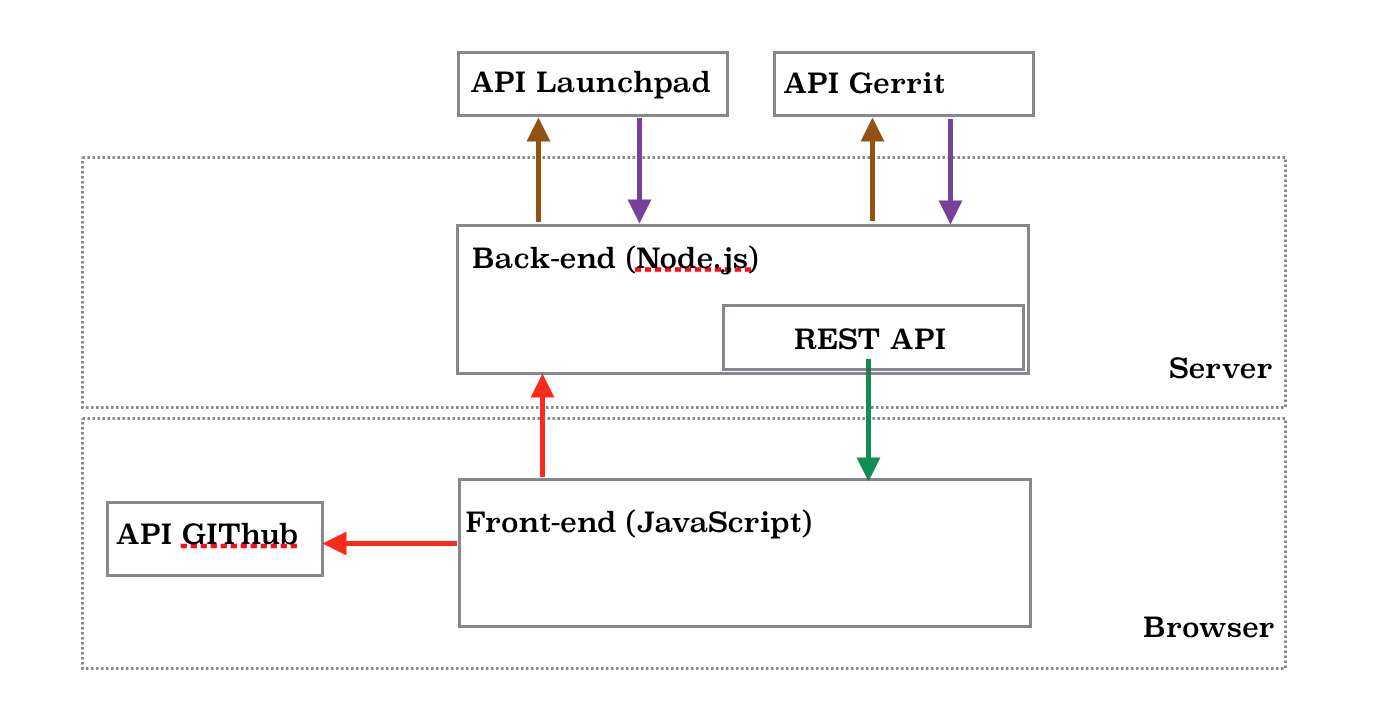
\includegraphics[height=7cm]{Arquitectura.png}
\caption{Architecture of the tool.}
\label{fig:1}       % Give a unique label
\end{figure}

\subsection{Main Features}
\label{sec:2.2}
The tool shows the id of the tickets, which are extracted randomly from each issue-tracking repository of OpenStack, and displays the information necessary to decide whether the issue is a bug report or not. We focused in display the main parameters that help in the classification, such as the title of the report and the description as well as the description of the fix commit.

The left side in the figure \ref{fig:2}, shows the information related with the ticket in Launchpad and its corresponding review in Gerrit. (FIXME: The two subsequent sentences are very strange and hard to understand, should really be rephrased for clarity.)Some information displayed link with the original web pages in Launchpad and Gerrit, thereby the developers have at their disposal extra information such as the comments that other developers have done. Could tracking the history since the ticket opens until the commit fixed the ticket. ( Is this way better? The developer can access to the Launchapd and Gerrit web pages through the links displayed in tool, thereby the developers can have extra information such as the comments that other developers have done in Launchpad or gerrit. This way, they could track the history of the ticket since it was open until the fix commit closed it. )

The right side is guided to user's opinion, after reading all the information displayed, they have to classify the ticket as \textit{Bug report} or \textit{Not Bug report}. Due to unsophisticated description used in the ticket, the developers could doubt in the classification, for this reason we add an extra option in the classification, \textit{Undecided}. Furthermore, the developers have a textarea to write their opinion about their classification in each ticket, as well as other textareas to write the keywords found in the title and the description which can help us building an automatic classification system in the future.

The tool allow carry out a blind analysis, meaning that the analysis can be done by two or more developers in parallel since the data is saved in a file in GitHub user's account. GitHub is a control version system in which we have access to all information of each commit submitted by the developer. Thus, saving the data in GitHub, we could measure the time that each developer spends in the analysis, which tickets were more difficult to analyze and other statistics that can help us in understanding the current problem of issue misclassification.

\begin{figure}
\centering
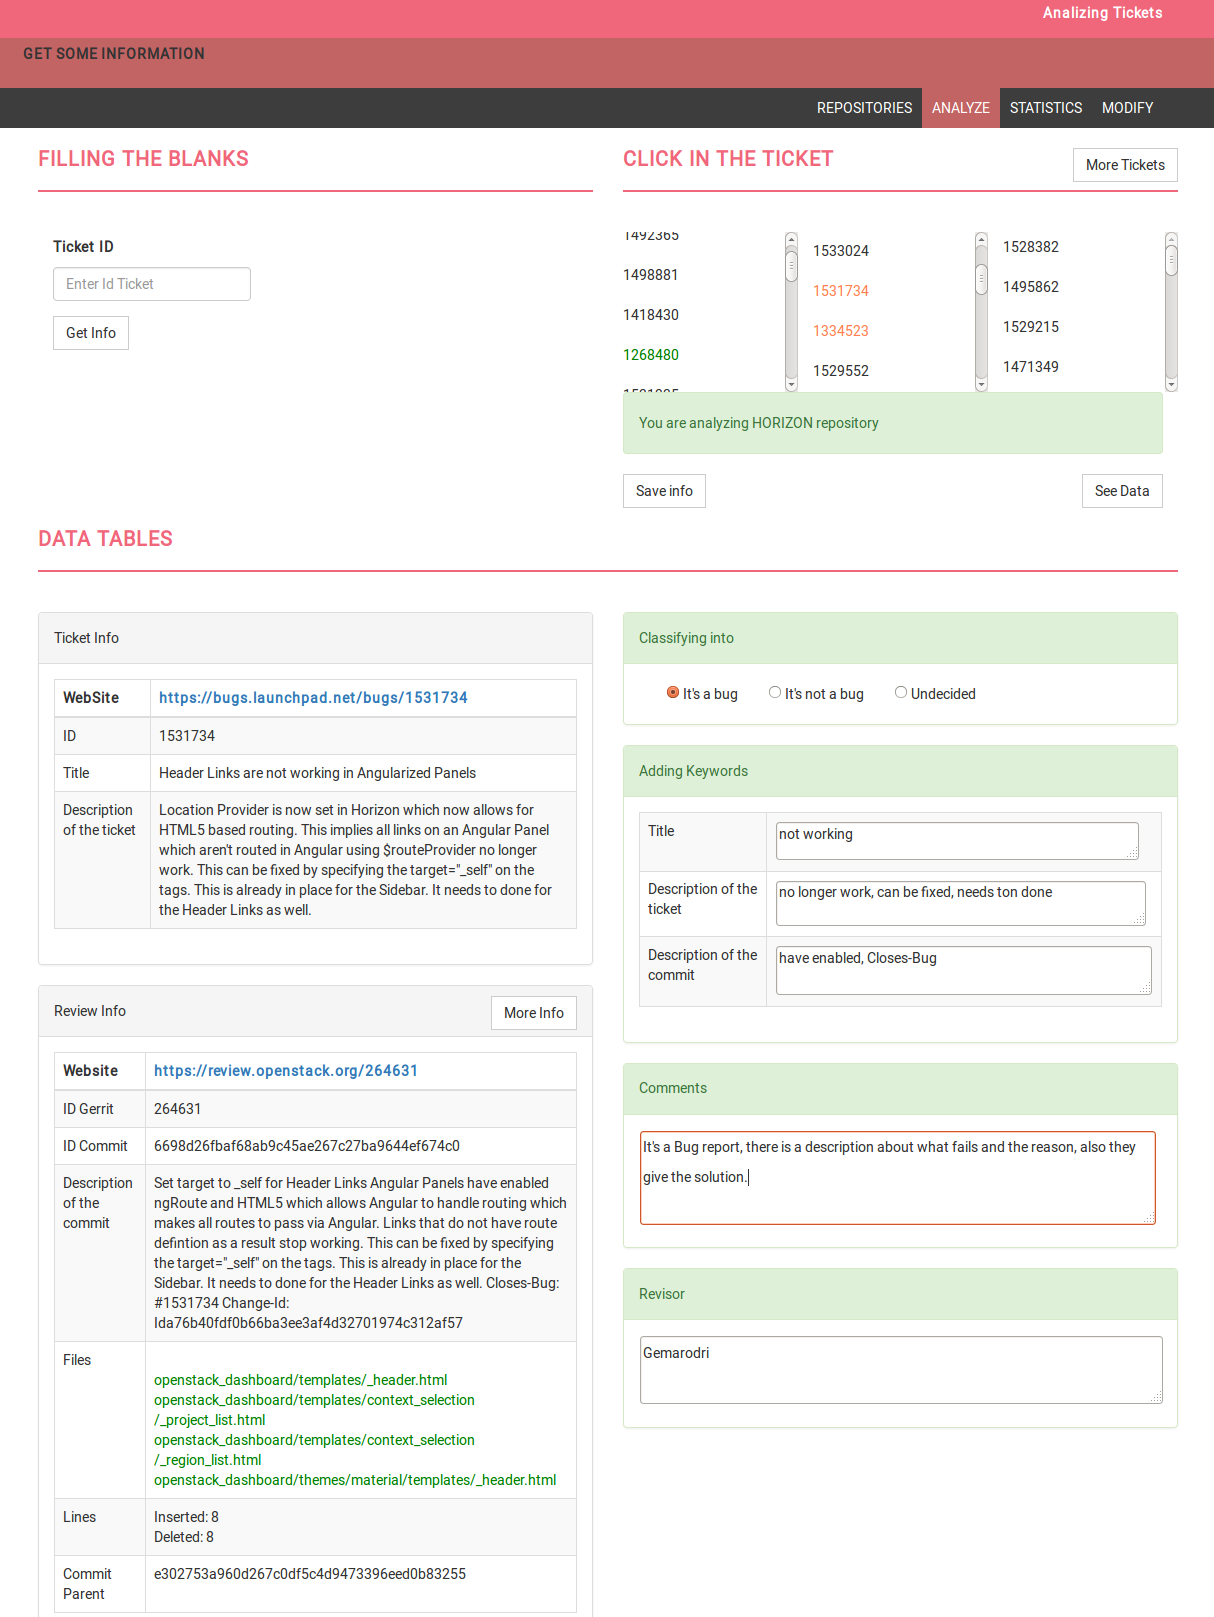
\includegraphics[height=19cm]{index2.png}
\caption{Screenshot of Analyze Tab}
\label{fig:2}       % Give a unique label
\end{figure}

The web page provides different functionalities depending on in which tab we are. Next we explain these functionalities.
\begin{enumerate}
  \item Tab Repository: In this tab we choose which repository of OpenStack we want analyze. Currently the tool supports the four principal repositories: Cinder, Nova, Neutron and Horizon.
  \item Tab Analyze: Is the Tab showed in Figure \ref{fig:2} where the user selects/inserts an identifier of a ticket and analyze with all the data displayed if the ticket is a bug report or not.
  \item Tab Statistics: This tab extracts the data already, analyzed by each developer involved in the analysis, from their users' accounts in GitHub. It analyzes this data to display a table with the number of tickets classified into the three categories; \textit{Bug Report},\textit{Not Bug Report} and \textit{Undecided}. To display the statistics of a developer, previously the name of developer has to be selected.
  \item Tab Modify: In this tab, the user can see the data saved in his GitHub repository and modify the content of the file that he wants, in case of have inserted a mistake during the analysis.
\end{enumerate}

We continue developing the tool but an initial version is available\footnote{\url{bugtracking.libresoft.es}}, as well as a demonstration video\footnote{\url{https://www.youtube.com/watch?v=q0-TIvL4mqc&feature=youtu.be}}. It presents a license type GPL 0 (General Public License) and you can find the code at a GitHub page\footnote{\url{https://github.com/Gemarodri/BugTracking}}. Anyone can use it regardless of having GitHub account or not. (FIXME: Language needs to be improved in remainder of this para.) But, only the ones with GitHub account can use the GitHub available functionalities; saved the data analyzed, see the statistics and modified the data saved. The one requirement is open a repository in GitHub with the same name that the project you want to analyze in OpenStack.

%\section{Validation Study}
%\label{sec:3}

%OpenStack was particularly of interest because of its highest scope and heterogeneous nature with hundreds of developers contributing, furthermore due to its short life, only 5 years, all history is saved and available in a version control system. The issues are called tickets in OpenStack and available in the Launchpad, a web interface of ticket tracking system, classifying them as bug report or not.

%We use the tool to analyze 500 randomly tickets from the four principal repositories in OpenStack. This tickets could be tagged as either "Fix Commited" or "Fix Released", to be able to localize the patch implemented into de source code in the version repository. They are generally tracked in Launchpad \texttt{Nova},\texttt{Cinder},\texttt{Horizon} and \texttt{Neutron}\footnote{\url{https://bugs.launchpad.net/NameOfRepository}}

%The parameters analyzed for each ticket were the title and the description of the report and the description of the fix commit. Also, the code changes if neither the descriptions and the comments clarified the underlying ticket. Each ticket was then categorized into one of three following groups.
%\begin{enumerate}
%  \item The ticket describes a bug report.
%  \item The ticket describes a feature, an optimization code, changes in test files or other not bug reports.
%  \item The ticket presents a vague description and cannot be classified without doubts.
%\end{enumerate}

%Henceforth, we will refer to Group 1 as \textit{Bug Report}, Group 2 as \textit{not Bug Report} and Group 3 as \textit{Undecided}.

%To validate the tool three different developers analyzed tickets belongs to the four main repositories. The developers analyzed more than four hundred tickets to can probe than the tool work as them expected, classifying the tickets into one of the three groups and corroborating that the issues reports present misclassification as ~\cite{Herzig} mentioned.

%In the analysis, some of the tickets present a double bind review process, obtaining that each tickets was analyzed by two developers. %Each developer analyzed 167 tickets plus the half tickets of his teammates. %Only at the end, they discussed the classification conflicts to reach an agreement.

\section{Results}
\label{sec:4}
(FIXME: (Review)The test of the tool in section 3 involves three developers use of the tool in order to identify which issues are perceived as bug reports. My concern (or observation) is that it is not obvious that the results primarily are connected to the tool (but rather use of the tool), i.e. it could be claimed that the actual object(s) of study are the developers and how similarly the perceive issues being bug reports. What would the results look like if the tool was not used (but rather the data sources in isolation) or some other possible tool? I am not saying that the test/investigation is without value, but I think this should be discussed somewhere in the paper.
)
We have manually analyzed 459 different tickets with support of the present tool, 125 from Cinder, 125 from Nova, 125 from Horizon and 84 from Neutron. All the tickets have been analyzed by two of the three developers and the Table ~\ref{tab:1} shows the percentage of tickets classified as bug reports for the different developers. These results don't report for some combinations of developers because of  in some projects, only a developer analyzed all the tickets and the two remaining analyzed the half of these tickets each one.   (FIXME: Discuss (more clearly) why results are not reported in Table 2 for combinations "D1 and D3" for Nova, "D2 and D3" for Horizon, and "D1 and D2" \& "D2 and D3" for Neutron.)
\begin{table}[htb]
\begin{center} {\footnotesize
\caption{ Classification statistics of each developer}
\label{tab:1}
\begin{tabular}{lllll}
\toprule[0.3mm]%{\smallskip}
  & Bug Report\kern 1pc & Not Bug Report\kern 1pc & Undecided\kern 1pc & Total \\\hline
Developer 1 \kern 1pc & (184) 55\% & (115) 34\% & (35) 11\% & 334 \\
Developer 2 \kern 1pc & (188) 76\% & (54) 22 \% & (7) 3\% & 249 \\
Developer 3 \kern 1pc & (188) 56\% & (116) 35\% & (30) 9\% & 334 \\
\bottomrule[0.3mm]
\end{tabular} }
\end{center}
\end{table}

The percentages between Developer 1 and Developer 3 are really similar, whereas the Developer 2 has identified more Bug Reports in his analysis. But, the three results support the misclassification present in bug tracking systems. Furthermore, according to ~\cite{Herzig}'s work, approximately two of five issues are misclassified in the analysis of Developer 1 and Developer 3.

Focusing in the concordance between developers analyzing the same ticket, 417 tickets present a double bind review process, obtaining that each ticket was analyzed by two developers. Table ~\ref{tab:2} shows the percentage of concordance between developers in each repository after the analysis of the tickets. Some repositories do not present double bind between two of developers.

\begin{table}[htb]
\begin{center} {\footnotesize
\caption{ Concordance between each developer in each repository}
\label{tab:2}
\begin{tabular}{llllll}
\toprule[0.3mm]%{\smallskip}
  & Nova\kern 1pc & Cinder\kern 1pc & Horizon\kern 1pc & Neutron\kern 1pc & Total\\\hline
D1 and D2  \kern 1pc & (44/63) 70\%\kern 1pc & (40/52) 77\%\kern 1pc & (37/62) 60\%\kern 1pc & - \kern 1pc& 68\% \\
D1 and D3  \kern 1pc &  -\kern 1pc & (46/63) 73\%\kern 1pc & (48/63) 76\%\kern 1pc & (26/42) 62\%\kern 1pc & 71 \% \\
D2 and D3  \kern 1pc & (41/62) 66\%\kern 1pc & (10/10) 100\%\kern 1pc  & - \kern 1pc& -\kern 1pc  &  71\% \\
\bottomrule[0.3mm]
\end{tabular} }
\end{center}
\end{table}

Table ~\ref{tab:2} shows that the concordance of the developers is high but, also demonstrate the difficulty to classify tickets as bug report or as not bug report, because each developer can have different ideas about a specific ticket. The concordance between the developers could be higher if they were expert in the project.
 
All the data iis available in the GitHub repositories of the developers \footnote{\url{https://github.com/Gemarodri}}\footnote{\url{https://github.com/ddalipaj}}\footnote{\url{https://github.com/nellysek}}, these repositories have the same name that the projects analyzed in OpenStack.

%\section{Discussion}
%\label{sec:5}

%Once we have all the tickets analyzed by diferents developers who have used a double blind, how to proceed if there are discordances between them:
%\begin{enumerate}
%\item Should they discuss after their analysis to reach a better classification?, Should the tool provide this?
%\item Does the Bug report only the same ticket classified as Bug report for all the developers?
%\end{enumerate}


\subsection{Future Work}
\label{sec:5.1}

%We would like know what grade of responsibility, none or totally, practice the previous commit in the seeding of a bug in OpenStack, considering that currently exists an implicit assumption: the line that contains the error was caused by the immediately previous commit\cite{Sliwerski}. The accuracy in our results depends on the quality of the data, thus we should focus only on bug reports discarding the other issues.

%The next step in the tool is implement the part in where we analyzed the previous commit, displaying the code after and before the bug fixed and after and before the bug-introduction to determinate if the previous commit is responsible or not.
(FIXME: This section needs to be linguistically improved)
The current tool is limited to OpenStack projects due to we are carrying out an empirical study which based on these data, but future extensions of this tool includes extract issues from others systems as Bugzilla or GitHub to study the misclassification in the OSS projects which use these systems. Also, display to users more information such as the code of the files affected in the fix commit, and the code in the bug seeding moment. Furthermore, we would like to implement an auto classifier based on the semantic of the ticket description and fix-commit description to help developers in the analysis. This classifier will show a percentage of confident about whereas the ticket belongs to bug report or not, but the developer always has the last decision. After manually analyzing more than 400 tickets, we have seen clear cases of issues that were bug reports, which have similar sentences in the description, so the automatic classification will allow developers to focus only on problematic issues, which can be easily misclassified. \\
(FIXME: it is understood that the current version of the tool is limited to Openstack projects/services and with the server operating against Launchpad and Gerrit. How well can the tool support other OSS projects through use of other kinds of repositories. This is hinted in 3.1 )\\
(FIXME: There are three styles specifying authors in the reference list. Make it uniform and conformant with the Springer conference paper requirements. Do not use "et al." in reference list, list all authors. For references 1 and 2 the source is not specified.
)

\begin{thebibliography}{4}

\bibitem{Antoniol}Antoniol, G., Ayari, K., Di Penta, M., Khomh, F., \& Gu\'eh\'eneuc, Y. G. (2008, October). Is it a bug or an enhancement?: a text-based approach to classify change requests. In Proceedings of the 2008 conference of the center for advanced studies on collaborative research: meeting of minds (p. 23). ACM.
\bibitem{Herzig}Herzig, K., Just, S., \& Zeller, A. (2013, May). It's not a bug, it's a feature: how misclassification impacts bug prediction. In Proceedings of the 2013 International Conference on Software Engineering (pp. 392-401). IEEE Press.
\bibitem{Sliwerski}J. Śliwerski, J., Zimmermann, T., \& Zeller, A. (2005, May). When do changes induce fixes?. In ACM sigsoft software engineering notes (Vol. 30, No. 4, pp. 1-5). ACM.
\bibitem {Nguyen}Nguyen, A. T., Nguyen, T. T., Nguyen, H. A., \& Nguyen, T. N. (2012, November). Multi-layered approach for recovering links between bug reports and fixes. In Proceedings of the ACM SIGSOFT 20th International Symposium on the Foundations of Software Engineering (p. 63). ACM.
\bibitem {Zimmermann}Zimmermann, T., Premraj, R., \& Zeller, A. (2007, May). Predicting defects for eclipse. In Predictor Models in Software Engineering, 2007. PROMISE'07: ICSE Workshops 2007. International Workshop on (pp. 9-9). IEEE.
\bibitem{Thomas}Zimmermann, T., \& Weißgerber, P. (2004, May). Preprocessing CVS data for fine-grained analysis. In Proceedings of the First International Workshop on Mining Software Repositories (pp. 2-6). sn.
\bibitem{Bird}Bird, C., Bachmann, A., Aune, E., Duffy, J., Bernstein, A., Filkov, V., \& Devanbu, P. (2009, August). Fair and balanced?: bias in bug-fix datasets. In Proceedings of the the 7th joint meeting of the European software engineering conference and the ACM SIGSOFT symposium on The foundations of software engineering (pp. 121-130). ACM.
\bibitem{NguyenTH}Nguyen, T. H., Adams, B., \& Hassan, A. E. (2010, October). A case study of bias in bug-fix datasets. In Reverse Engineering (WCRE), 2010 17th Working Conference on (pp. 259-268). IEEE.
\end{thebibliography}

\end{document}
